%%\def\beginanswers{\iffalse}
\def\beginanswers{\iftrue}

\documentclass[10pt]{article}
\usepackage{amsmath,amsfonts,amsthm,amssymb}
\usepackage{graphicx}
\usepackage{enumerate}
\usepackage{upquote,textcomp}
\usepackage{listings}
\usepackage{color}

\definecolor{mygreen}{rgb}{0,0.6,0}
\definecolor{mygray}{rgb}{0.5,0.5,0.5}
\definecolor{mymauve}{rgb}{0.58,0,0.82}


\lstset{frame=tb,
  language=,
  aboveskip=3mm,
  belowskip=3mm,
  showstringspaces=false,
  columns=flexible,
  keepspaces=true,
  basicstyle={\small\ttfamily},
  numbers=none,
  numberstyle=\tiny\color{black},
  keywordstyle=\color{black},
  commentstyle=\color{black},
  stringstyle=\color{black},
  breaklines=true,
  breakatwhitespace=true,
  tabsize=3
}

\lstset{frame=tb,
  language=Python,
  aboveskip=3mm,
  belowskip=3mm,
  showstringspaces=false,
  columns=flexible,
  basicstyle={\small\ttfamily},
  numbers=none,
  numberstyle=\tiny\color{mygray},
  keywordstyle=\color{blue},
  commentstyle=\color{mygreen},
  stringstyle=\color{mymauve},
  breaklines=true,
  breakatwhitespace=true,
  tabsize=3
}


\newcommand{\vect}[1]{{\bf #1}}                 %for bold chars
\newcommand{\vecg}[1]{\mbox{\boldmath $ #1 $}}  %for bold greek chars
\newcommand{\matx}[1]{{\bf #1}}

\setlength{\parindent}{0in}
\setlength{\parskip}{1em}
\setlength{\textheight}{9.5in}
\setlength{\textwidth}{7in}
\setlength{\headsep}{0in}        % distance from top of page to address
\setlength{\topmargin}{-0.5in}
\setlength{\oddsidemargin}{-0.5in}
\setlength{\evensidemargin}{-0.5in}


\begin{document}
\thispagestyle{empty}

\vspace*{0.5in}

\begin{center}
\Large
\textbf{Open Source Software --- CSCI-4470 --- Spring 2022} \\
\textbf{Test 1} \\
\textbf{March 5, 2021}
\end{center}


%%%%%%%%%%%%%%%%%%%%%%%%%%%%%%%%%%%%%%%%%%%%%%%%%%%%%%%%%%%%%%%%%%%%%%%%
%%%%%%%%%%%%%%%%%%%%%%%%%%%%%%%%%%%%%%%%%%%%%%%%%%%%%%%%%%%%%%%%%%%%%%%%
\beginanswers
\begin{center}
\Large
\textbf{SOLUTIONS}
\end{center}

%%%%%%%%%%%%%%%%%%%%%%%%%%%%%%%%%%%%%%%%%%%%%%%%%%%%%%%%%%%%%%%%%%%%%%%%
\else
%%%%%%%%%%%%%%%%%%%%%%%%%%%%%%%%%%%%%%%%%%%%%%%%%%%%%%%%%%%%%%%%%%%%%%%%


\begin{center}

\textbf{\Large Name:} \underline {\hspace{2.0in}} \\

\bigskip
\bigskip

\centerline{
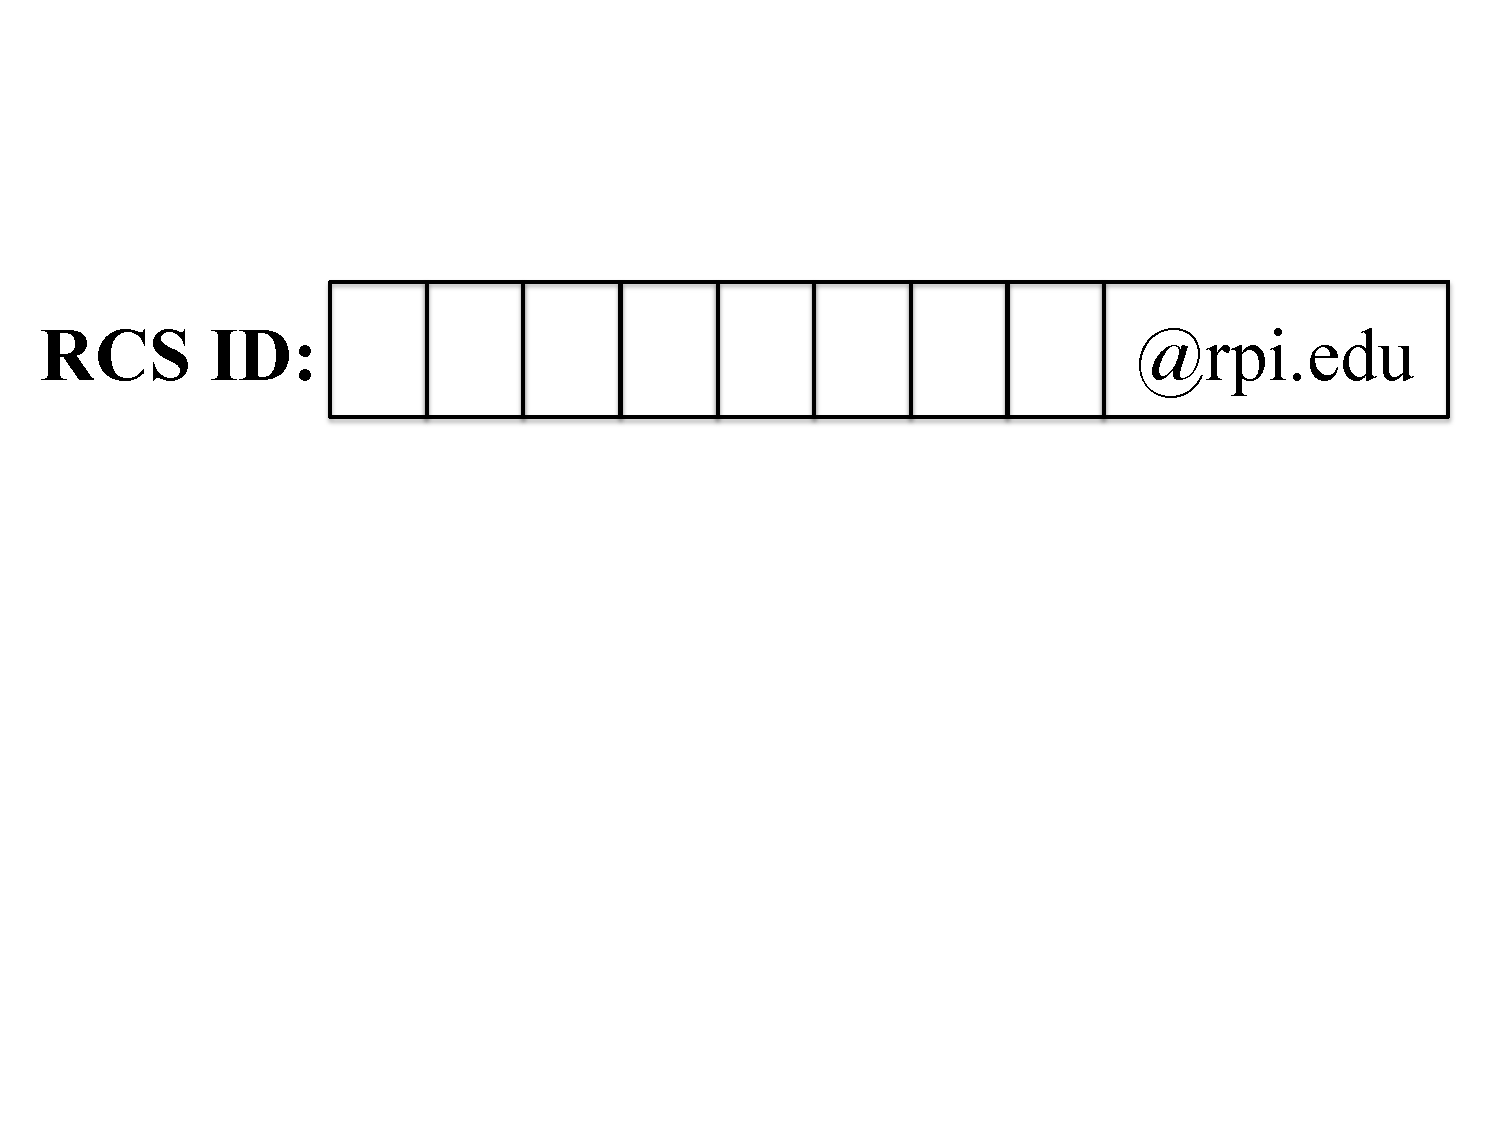
\includegraphics[height=0.5in]{boxes}
}

%%  \begin{tabular}{|p{0.1in}|p{0.1in}|p{0.1in}|p{0.1in}|p{0.1in}|p{0.1in}|p{0.1in}|p{0.1in}|l|}
%%    \hline \\
%%   & & & & & & & & \textbf{\large @rpi.edu} \\
%%  \hline
%%  \end{tabular} 
%%  
%%  \end{tabular}

\bigskip

\textbf{\Large RIN\#:} \underline {\hspace{1.5in}}  

\vspace*{0.4in}
{\large\bf Honor pledge: On my honor I have neither given
nor received aid on this exam.}

\vspace*{0.1in}
{\large\bf Please sign here to indicate that you agree with the honor pledge: \underline {\hspace{1.5in}}}
\end{center}

\vspace*{.45in} 

{\large\bf Instructions:}
\begin{itemize}
%%\item You have 90 minutes to complete this test.
\item Clearly print your name, RCS ID (in all caps.) and your RIN at the top of your exam.
\item This test is open book, open notes and open computer. You {\textbf may not} use the internet. Please turn off your wifi.
\item There are \textbf{6 questions} on this test worth a total of
  \textbf{100 points}.
\end{itemize}

\centering{\begin{tabular}{|c|c|r|}
	\hline
	Question & Score & Possible \\ \hline
	1 &  & 15 \\ \hline
	2 &  & 14 \\ \hline
	3 &  & 15 \\ \hline
	4 &  & 15 \\ \hline
	5 &  & 18 \\ \hline
	6 &  & 23 \\ \hline
	Total &  & 100 \\ \hline
\end{tabular}}

\newpage

%% ^\d?[\( ]?(\d{3})[- \)]*\d{3}[- \)]*\d{4}

%%%%%%%%%%%%%%%%%%%%%%%%%%%%%%%%%%%%%%%%%%%%%%%%%%%%%%%%%%%%%%%%%%%%%%%%
\fi
%%%%%%%%%%%%%%%%%%%%%%%%%%%%%%%%%%%%%%%%%%%%%%%%%%%%%%%%%%%%%%%%%%%%%%%%

\begin{enumerate}
	%% Spring 2022
	\item Give regex expressions for each of the following (15 pts)
	
	\beginanswers
		\begin{enumerate}[1]
		\bigskip
		\item \verb|^[a-z]{3,6}[0-9]*@rpi\.edu|
		\bigskip
		\item \verb!^(518|\(518\)\s*|518(\-| ))276(\-| )*[0-9]{4}$!
		\bigskip
		\item \verb|110 Eighth St\.\N*Troy\N*NY\N*12180|
		\end{enumerate}
	\else
		
		\begin{enumerate}[a]
		\bigskip
		\item Given a list of strings, one per line, recognize an RPI email address. Note that an RPI email address has the form rcsid@rpi.edu, where \verb|rcsid| is between 3 and 6 alphabetic characters followed by 0 or more digits. All other strings should not be recognized. (Note that \verb|pattern{lower, upper}| recognizes between lower and upper repetitions of  pattern. I.e. \verb|a{2,3}| recognizes \verb|aa| and \verb|aaa|) . You can assume each email starts at the beginning of the line.
		
		Given:
		
		\begin{verbatim}
			turnew2@rpi.edu
			re@rpi.edu
			turnerw2@rpi.edu
			turnew@rpi.edu
		\end{verbatim}
		
		The expression should recognize \verb*|turnew2@rpi.edu| and \verb*|turnew@rpi.edu|
		\bigskip
		\bigskip
	\bigskip
	\bigskip
		\bigskip
	\bigskip
	\bigskip
		\bigskip
		\bigskip
	\bigskip
\bigskip
\bigskip
		\item RPI has a campus in Troy, NY with an area code 518 and a prefix 276. The last 4 digits are arbitrary. Write a regular expression to recognize any sequence of 10 digits that can be interpreted as a valid RPI phone number. It should handle 10 consecutive digits with the correct area code and prefix, it should handle the area code in parentheses, or it should handle area code, prefix and number separated by dashes, spaces or a combination of both, For example, the regex should recognize all of:
		
\begin{verbatim}
5182769999
(518) 276-9999
518-276-9999
518 276 9999
518276 9999
\end{verbatim}

but not:

\begin{verbatim}
518(276)(9999)
518-276-09999
518)2769999		
\end{verbatim}

You can assume each phone number starts at the beginning of the line.
		
		\bigskip
		\bigskip
	\bigskip
	\bigskip
		\bigskip
	\bigskip
	\bigskip
		\bigskip
		\bigskip
		
		\newpage
		
		\item Finally, recognize every line that has RPI's street address of \verb|110 Eighth St., Troy, NY 12180| the strings ``110 Eighth St.'', `` Troy'', ``NY'' and ``12180'' must appear in order, but can be separated by an arbitrary number of other characters and whitespace so long as it is on the same line.
		
		Your program should recognize:
		
		\begin{verbatim}
		RPI 110 Eighth St. Troy, NY 12180
		RPI 110 Eighth St. Lally Building, Troy              NY    12180
		\end{verbatim}
	
	But not:
	
		\begin{verbatim}
	RPI 111 Eighth St. Troy, NY 12180
	RPI 110 Eighth Troy St. Lally Building, Troy              NY    12180
	RPI 12180 110 Eighth St. Lally Building, Troy              NY 
\end{verbatim}

	
		
		\bigskip
		\bigskip
	\bigskip
\bigskip
\bigskip
	\bigskip
\bigskip
\bigskip
		\bigskip
			\end{enumerate}
		\fi
	
\newpage


	\item For each of the following licenses, indicate whether the license is ``Copyleft'', ``Weak Copyleft'', ``Permissive'', or Not an Open Source/Free Software License. Circle the best answer. (14 pts.)
	 	
\beginanswers
\begin{enumerate}[a]
	\item \textbf{MPL}

\begin{enumerate}[A.]
	\item Copyleft
	\item \textbf{Weak Copyleft}
	\item Permissive
	\item Not an Open Source/Free Software License
\end{enumerate}

\item \textbf{QaPL}

\begin{enumerate}[A.]
	\item Copyleft
	\item Weak Copyleft
	\item Permissive
	\item \textbf{Not an Open Source/Free Software License}
\end{enumerate}

\item \textbf{BSD}

\begin{enumerate}[A.]
	\item Copyleft
	\item Weak Copyleft
	\item \textbf{Permissive}
	\item Not an Open Source/Free Software License
\end{enumerate}

\item \textbf{AGPL}

\begin{enumerate}[A.]
	\item \textbf{Copyleft}
	\item Weak Copyleft
	\item Permissive
	\item Not an Open Source/Free Software License
\end{enumerate}

\item \textbf{LGPL}

\begin{enumerate}[A.]
	\item Copyleft
	\item \textbf{Weak Copyleft}
	\item Permissive
	\item Not an Open Source/Free Software License
\end{enumerate}

\item \textbf{MIT}

\begin{enumerate}[A.]
	\item Copyleft
	\item Weak Copyleft
	\item \textbf{Permissive}
	\item Not an Open Source/Free Software License
\end{enumerate}

\item \textbf{EPL}

\begin{enumerate}[A.]
	\item Copyleft
	\item \textbf{Weak Copyleft}
	\item Permissive
	\item Not an Open Source/Free Software License
\end{enumerate}
	
\end{enumerate}
\else
\begin{enumerate}[i.]
	\item \textbf{MPL}

	\begin{enumerate}[A.]
		\item Copyleft
		\item Weak Copyleft
		\item Permissive
		\item Not an Open Source/Free Software License
	\end{enumerate}

	\item \textbf{QaPL}

\begin{enumerate}[A.]
	\item Copyleft
	\item Weak Copyleft
	\item Permissive
	\item Not an Open Source/Free Software License
\end{enumerate}

	\item \textbf{BSD}

\begin{enumerate}[A.]
	\item Copyleft
	\item Weak Copyleft
	\item Permissive
	\item Not an Open Source/Free Software License
\end{enumerate}

\item \textbf{AGPL}

\begin{enumerate}[A.]
	\item Copyleft
	\item Weak Copyleft
	\item Permissive
	\item Not an Open Source/Free Software License
\end{enumerate}

\item \textbf{LGPL}

\begin{enumerate}[A.]
	\item Copyleft
	\item Weak Copyleft
	\item Permissive
	\item Not an Open Source/Free Software License
\end{enumerate}

\item \textbf{Apache}

\begin{enumerate}[A.]
	\item Copyleft
	\item Weak Copyleft
	\item Permissive
	\item Not an Open Source/Free Software License
\end{enumerate}

\item \textbf{LGPL}

\begin{enumerate}[A.]
	\item Copyleft
	\item Weak Copyleft
	\item Permissive
	\item Not an Open Source/Free Software License
\end{enumerate}

\end{enumerate}
\fi

\newpage

    \item Reconstruct the following page in MarkDown or Restructured Text . You may assume that the image is named \verb*|pexels-jennifer-murray-1067202.png| and is located in the same directory as this file. Write your answer on the next page. (18 pts):
    
    \centerline{
    	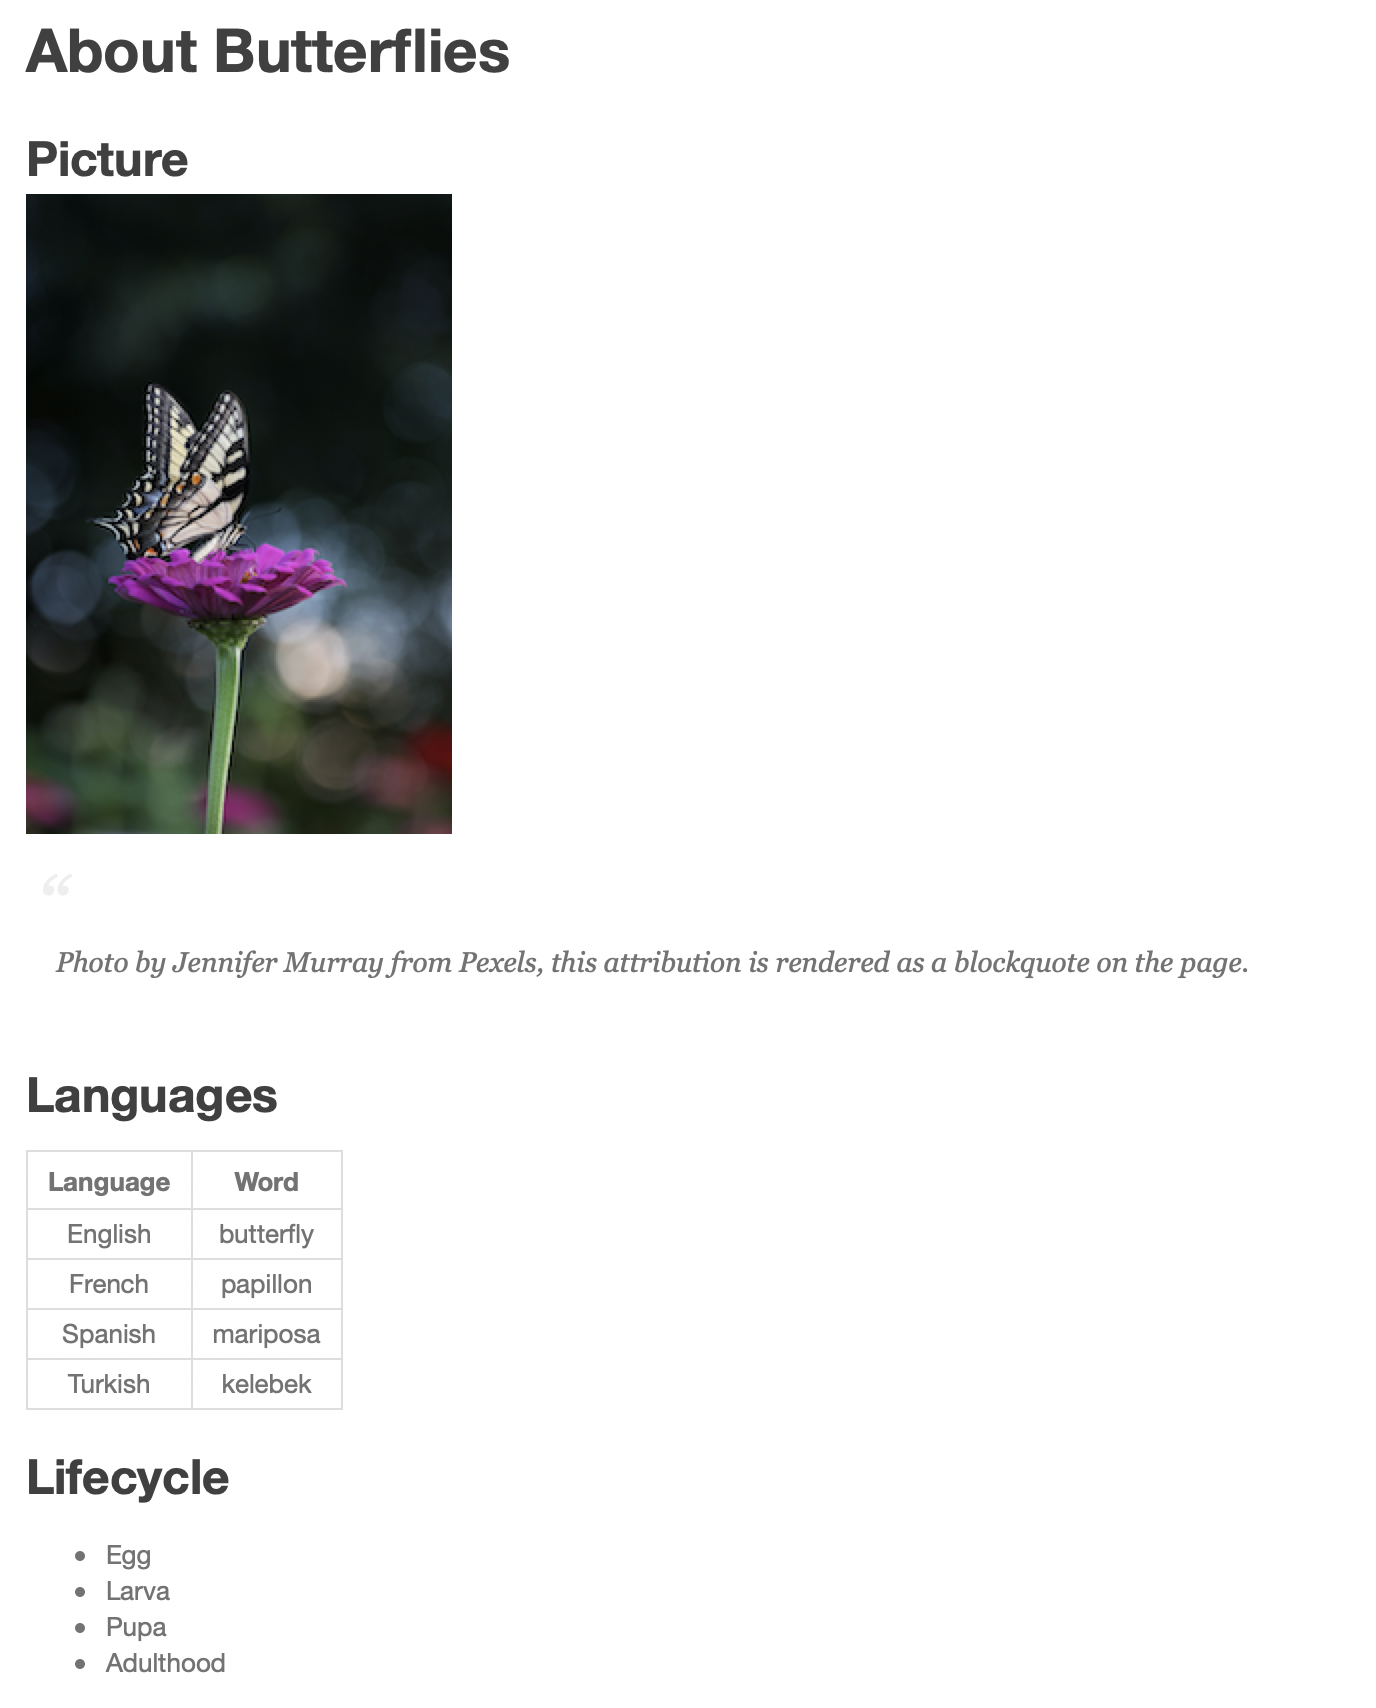
\includegraphics[width=6in]{page}
    }

\newpage
    
    \beginanswers
    \begin{lstlisting}
    	# About Butterflies
    	
    	Picture
    	-------
    	![](pexels-jennifer-murray-1067202.png)
    	
    	> Photo by Jennifer Murray from Pexels, this attribution is rendered as a blockquote on the page.
    	
    	Languages
    	---------
    	| Language | Word |
    	|:-----:|:-------:|
    	|English | butterfly|
    	| French| papillon|
    	|Spanish| mariposa|
    	|Turkish|kelebek|
    	
    	Lifecycle
    	-----
    	* Egg
    	* Larva
    	* Pupa
    	* Adulthood
    	\end{lstlisting}
    or
    \begin{lstlisting}
    	=================
    	About Butterflies
    	=================
    	
    	Picture
    	-------
    	
    	.. image:: pexels-jennifer-murray-1067202.png
    	
    	..
    	
    	*Photo by Jennifer Murray from Pexels, this attribution is rendered as a blockquote on the page.*
    	
    	..
    	Languages
    	---------
    	+----------+-----------+
    	| Language |    Word   |
    	+----------+-----------+
    	|  English | butterfly |
    	+----------+-----------+
    	|  French  |  papillon |
    	+----------+-----------+
    	|  Spanish |  mariposa |
    	+----------+-----------+
    	|  Turkish |  kelebek  |
    	+----------+-----------+
    	
    	Lifecycle
    	-----
    	* Egg
    	* Larva
    	* Pupa
    	* Adulthood
    	\end{lstlisting}
  \else
  \hspace*{-0.4in}\framebox(540,600){}
  \fi
  
  \newpage

\item Provide answers to the questions below. Your answers do not need to be long. A few sentences should be sufficient to capture the important points (15pts).

\begin{enumerate}
	\item In  \textit{The Cathedral and the Bazaar}, what principle (number and quote) does Eric Raymond dub \textbf{Linus' Law}?
	
	\beginanswers
	\textbf{\# 8 Given a large enough beta-tester and co-developer base, almost
	every problem will be characterized quickly and the fix obvious to
	someone.}
	\else
	\bigskip
	\bigskip
	\bigskip
	\bigskip
	\bigskip
	\bigskip
	\bigskip
	\bigskip
	\bigskip
	\bigskip
\bigskip
\bigskip
\bigskip
\bigskip
\bigskip
\bigskip
\bigskip
\bigskip
\bigskip
\bigskip
	\fi

	\item In  \textit{The Cathedral and the Bazaar}, what principle does Eric Raymond use to argue against writing code from scratch when existing software can be used or repurposed?


	\beginanswers	
\textbf{\# 2 Good programmers know what to write. Great ones know what
to rewrite (and reuse)}	
    \else
	\bigskip
	\bigskip
	\bigskip
	\bigskip
	\bigskip
	\bigskip
	\bigskip
	\bigskip
	\bigskip
	\bigskip
	\bigskip
	\bigskip
	\bigskip
	\bigskip
	\bigskip
	\bigskip
	\bigskip
	\bigskip
	\bigskip
	\bigskip
	\fi
	
	\item Discuss the major differences between a \textbf{copyleft} and a \textbf{permissive} software license. At what point of the software development lifecycle does this apply?
	
	\beginanswers
	While copyleft licenses differ in what they consider \textbf{derivative works}, all \textbf{copyleft} licenses require some type of reciprocity in how derivative works are licensed. Typically, this requires that derivative works be licensed under the same or at least a compatible copyleft license. A \textbf{permissive} license generally gives broad latitude to how derivative works are licensed. These differences only come into effect when software is distributed.
\else
\bigskip
\bigskip
\bigskip
\bigskip
\bigskip
\bigskip
\bigskip
\bigskip
\bigskip
\bigskip
\bigskip
\bigskip
\bigskip
\bigskip
\bigskip
\bigskip
\bigskip
\bigskip
\bigskip
\bigskip
\fi
\end{enumerate}
	
\newpage


\item Consider the following scenario. You have a fork of an open source library in github. You can assume that the original is at: \verb*|git@github.com:RCOS/project.git| and your fork is at \verb*|git@github.com:me/project.git|.

Show the sequence of git commands to do the following:
\begin{itemize}
	\item Establish a local repository based on your fork
	\item Establish remote links to the original github repository \textit{(upstream)} and to your fork \textit{(remote)}
	\item Create a branch (\textit{mybranch}) on your local repository
\end{itemize}

Now assume you have a modified file \textit{modified.txt} on your local repository complete the sequence by:

\begin{itemize}
	\item Get the changes to \textit{modified.txt} added to \textit{mybranch}
	\item Apply the changes in \textit{mybranch} and any changes made to the upstream master to your \textit{main}
	\item Make the main branch on your github fork consistent with your local main branch
\end{itemize}

You must use the command line for all git operations. (18 pts)

Write your git commands below

\beginanswers
\begin{lstlisting}
git clone git@github.com:me/project.git
git remote add origin git@github.com:me/project.git # Optional - clone should do it
git remote add upstream git@github.com:RCOS/project.git
git checkout -b mybranch
git add modified.txt
git commit -m "Changes" # message is arbitrary
git checkout main
git merge mybranch
git pull upstream main
git push remote main
\end{lstlisting}
\else
\hspace*{-0.4in}\framebox(540,460){}
\fi
\newpage

\item Consider build systems. Answer the following questions (23pts):

\begin{enumerate}
\item Write a \verb*|Makefile| that captures the relationship depicted in the depndency diagram below.  (16 of 23 pts).

\centerline{
	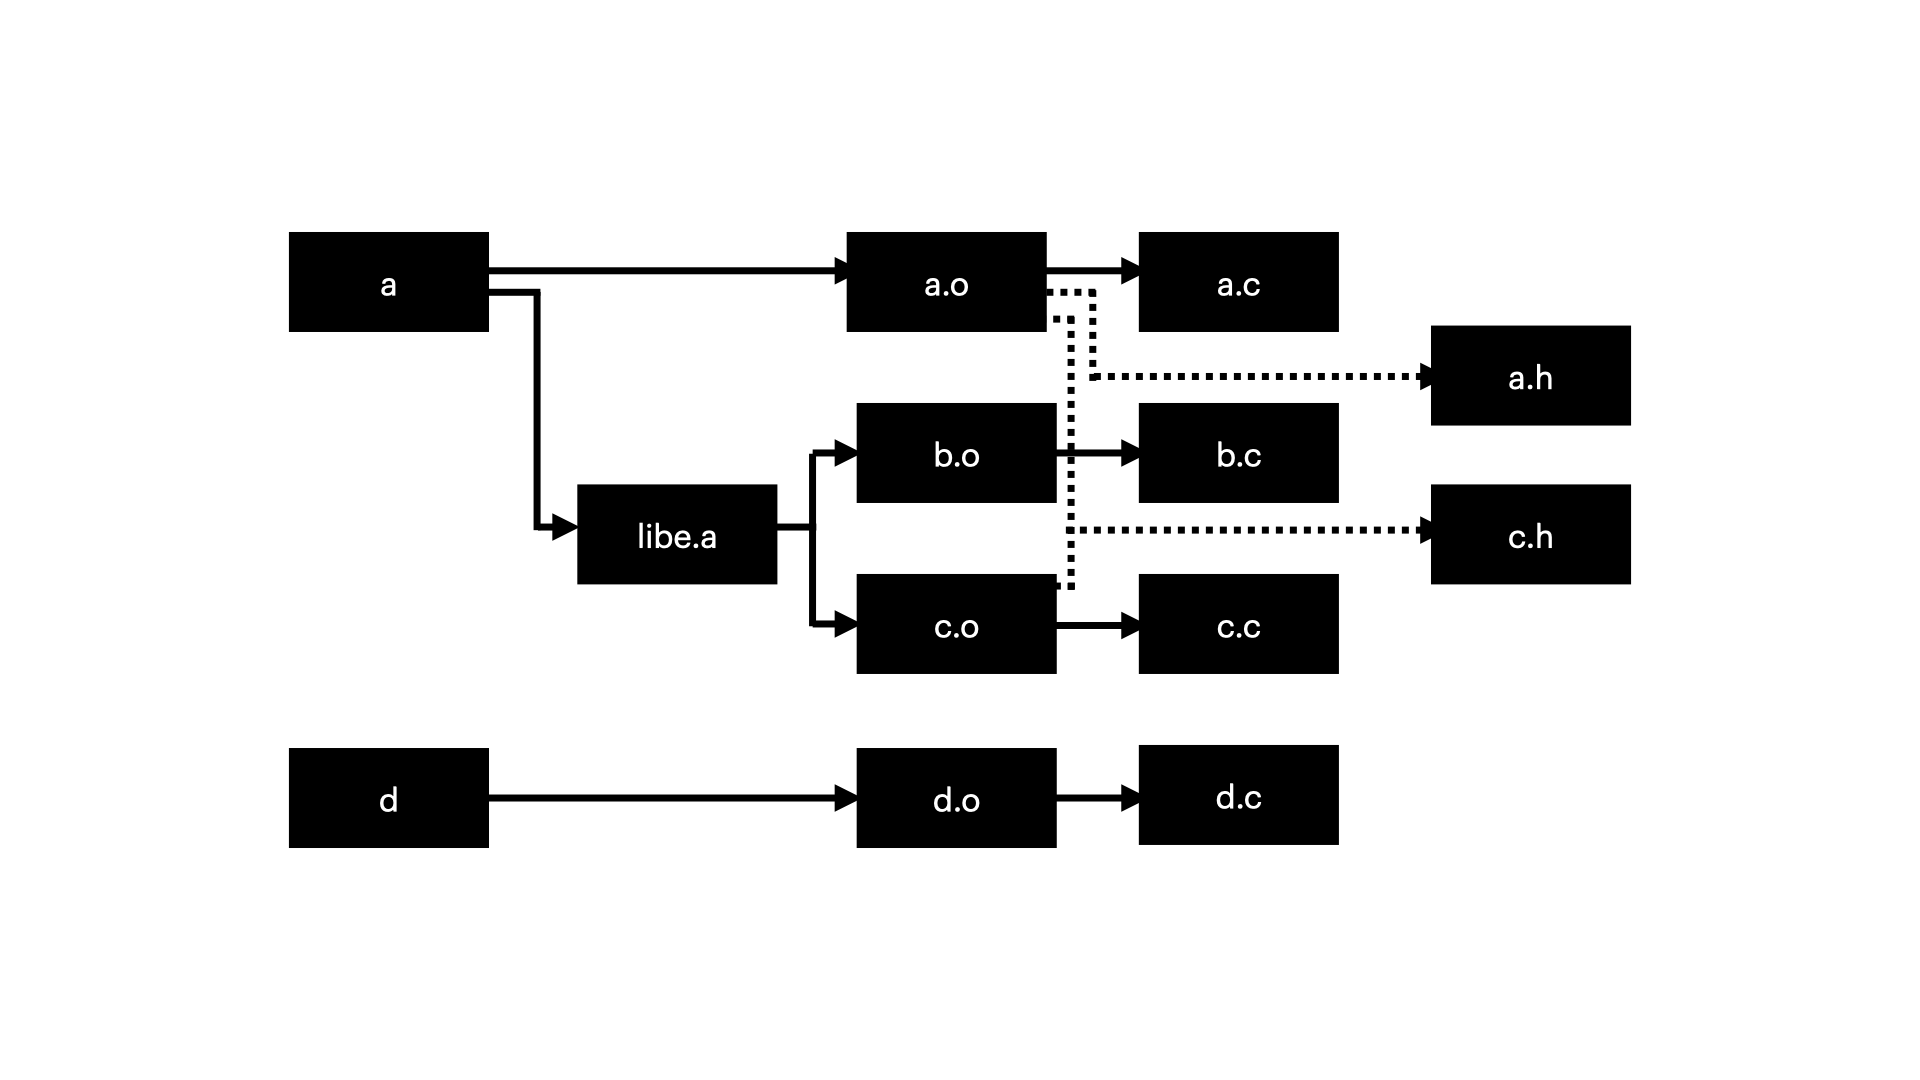
\includegraphics[width=7.5in]{dependency}
}
A few notes:
\begin{itemize}
	\item Do not use shortcuts. Put in the commands to create each object file and each library, etc. explicitly in the file.
	\item The \verb*|Makefile| must be hand generated. Do not use a Makefile generator (such as cmake) to create the file.
	\item Make sure you have \verb*|clean| and \verb|all| build targets.
\end{itemize}

\begin{center}
\LARGE\textbf{Write your Makefile on the next page.}
\end{center}

\beginanswers
\begin{lstlisting}[language=make]
all: a d

clean:
	rm a d libe.a a.o b.o c.o d.o 

a.o: a.c a.h c.h
	cc -c -o a.o a.c

b.o: b.c
	cc -c -o b.o b.c

c.o: c.c c.h
	cc -c -o c.o c.c

d.o: d.c
	cc -c -o d.o d.c

a: a.o libe.a
	cc a.o libe.a -o a

d: d.o
	cc d.o -o d

libe.a: b.o c.o
	ar qc libe.a b.o c.o

\end{lstlisting}
\else
\hspace*{-0.4in}\framebox(540,650){}
\fi
\newpage
	\item Now consider the CMakeLists file below. Add commands to the file to generate 3 tests.  (7 of 23 pts)
			
	\begin{itemize}
		\item Test 1 - Verify ``main'' runs
		\item Test 2 - Verify the usage information exists
		\item Test 3 - Verify that running main with 32 returns the value 18
	\end{itemize}

Here is the output of running ``main'':
\begin{lstlisting}
	>>> main
	Usage: main number
	>>> main 32
	18
\end{lstlisting}

\textbf{CMakeLists.txt} 
	\begin{lstlisting}
	cmake_minimum_required(VERSION 3.0)
	project(Main C)
	
	add_library(shared SHARED shared/shared.c)
	
	add_library(static STATIC static/static.c)
	
	add_executable(main main.c helper.c)
	target_link_libraries(main shared static)
	
	install(TARGETS shared DESTINATION lib)
	install(TARGETS main DESTINATION bin)
\end{lstlisting}

\beginanswers
\begin{lstlisting}[language=make]
cmake_minimum_required(VERSION 3.0)
project(Main C)

add_library(shared SHARED shared/shared.c)

add_library(static STATIC static/static.c)

add_executable(main main.c helper.c)
target_link_libraries(main shared static)

install(TARGETS shared DESTINATION lib)
install(TARGETS main DESTINATION bin)

enable_testing()

# does the application run
add_test(NAME Runs COMMAND main)

# does the usage message work?
add_test(NAME Usage COMMAND main)
set_tests_properties(Usage
PROPERTIES PASS_REGULAR_EXPRESSION "Usage:.*number"
)

# does the program work correctly?
add_test(NAME Test1 COMMAND main 32)
set_tests_properties(Usage
PROPERTIES PASS_REGULAR_EXPRESSION "18"
)

\end{lstlisting}
\else
Your additions. (Do not repeat the above lines.)

\hspace*{-0.4in}\framebox(540,370){}

\fi
\end{enumerate}
	
\end{enumerate}
\end{document}
